\documentclass{report}
\usepackage[margin=1in]{geometry}
\usepackage{amsmath}
\usepackage{amssymb}
\usepackage{subfiles}

\title{ENGT 3652 Project 5:\\*CNC Lathe-Bishop}
\author{Leomar Dur\'an}
\date{${25}^{\text{th}}$ April 2023}

\usepackage{pdflscape}
\usepackage{graphicx}
\usepackage{minted}
\newcommand*\gcode{lib/pygments/gcodelexer.py:GcodeLexer -x}

\usepackage[final]{pdfpages}
% compile the subfiles
\write18{
    % the manual gcode in two columns
    pdflatex gcode-manual
}
\write18{
    % the manual gcode for CNC Simulator in two columns
    pdflatex gcode-manual-for_cnc_simulator
}

\write18{
    % the manual gcode for CNC Simulator in two columns
    pdflatex gcode-cam
}

\begin{document}

\maketitle

\chapter{Original drawing}
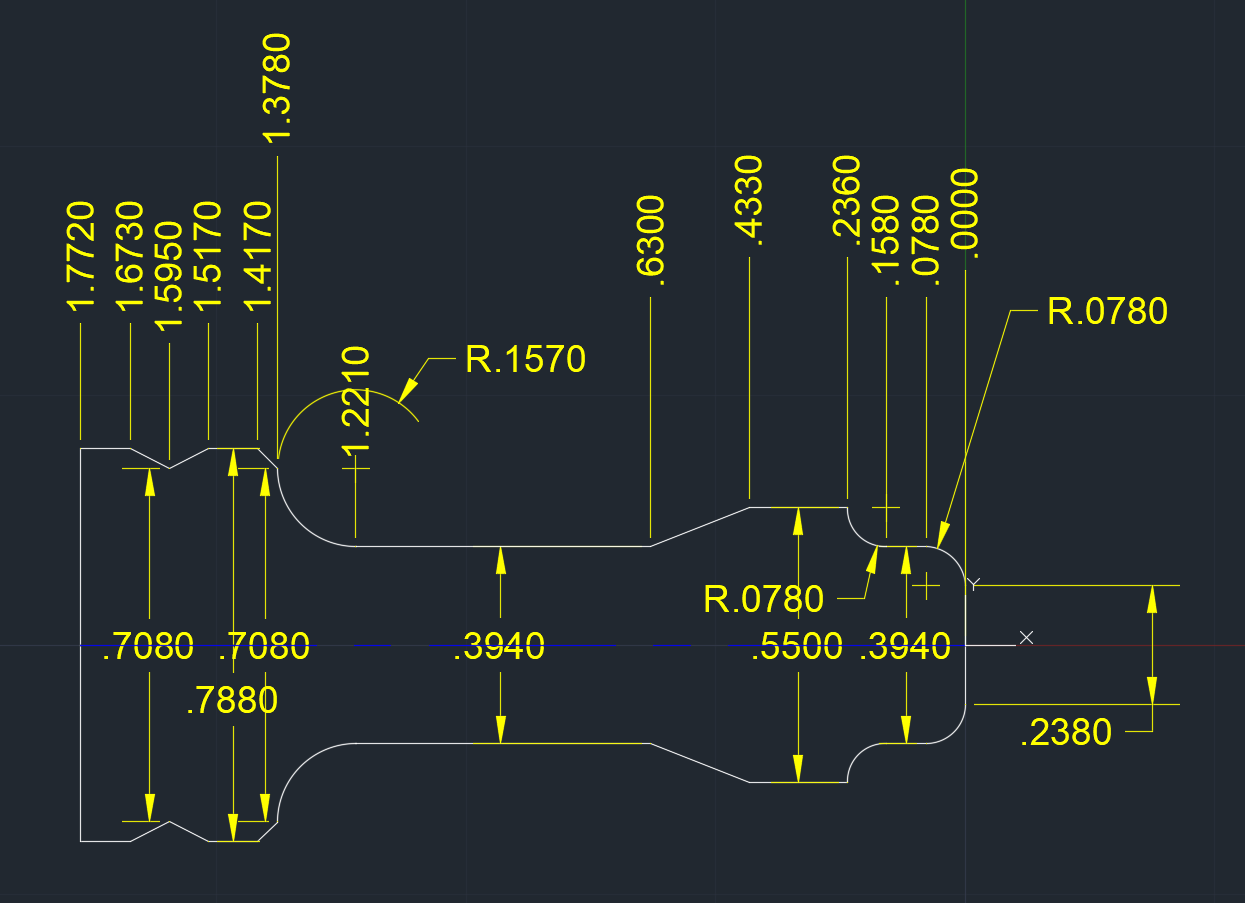
\includegraphics[width=\textwidth]{Bishop - The path_pptx/ppt/media/image1.png}

%\chapter{Path}
\addtocounter{chapter}{1}
\includepdf[landscape,pages=-,pagecommand={}]{Bishop - The path_pptx.pdf}

%\chapter{Gcode}
\addtocounter{chapter}{1}
\includepdf[pages=2-,pagecommand={}]{gcode-manual.pdf}

\chapter{Plot of manual Gcode in NCViewer}
\begin{landscape}
% this image has a lower portrait aspect ratio than a page, so use height for reference
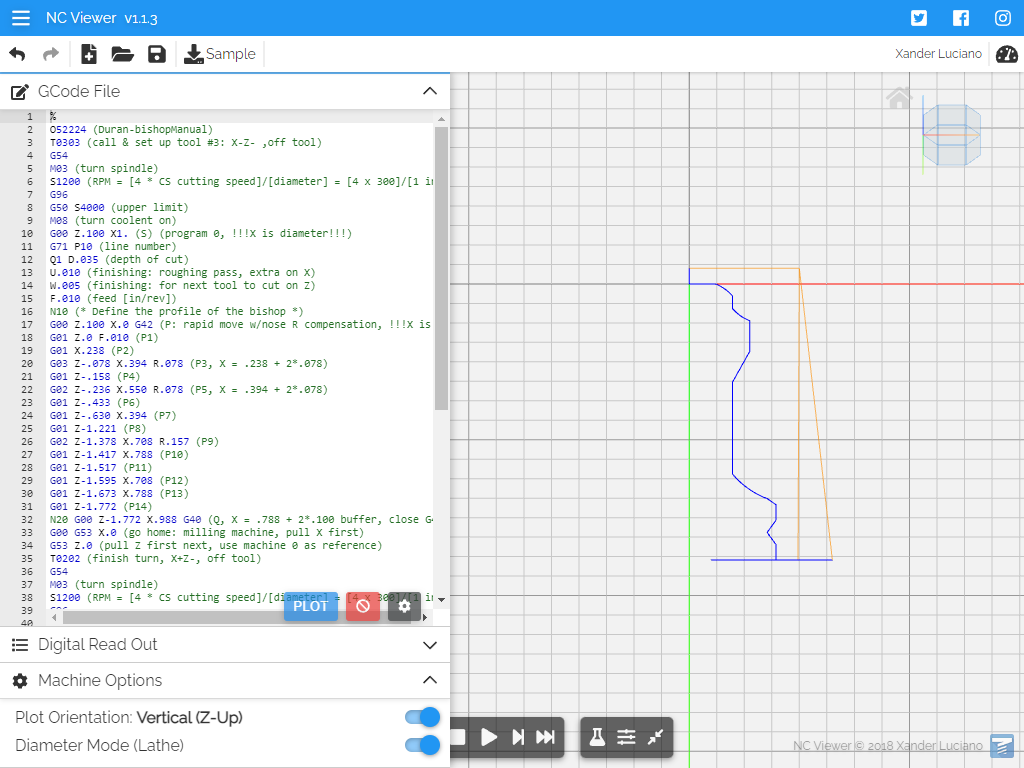
\includegraphics[height=\textheight]{img/prj05-manual-gcode-ncviewer-plot-xz.png}
\end{landscape}

%\chapter{Gcode for CNC Simulator}
\addtocounter{chapter}{1}
\includepdf[pages=2-,pagecommand={}]{gcode-manual-for_cnc_simulator.pdf}

\chapter{Result of manual Gcode for CNC Simulator}
\begin{landscape}
\null\vfill
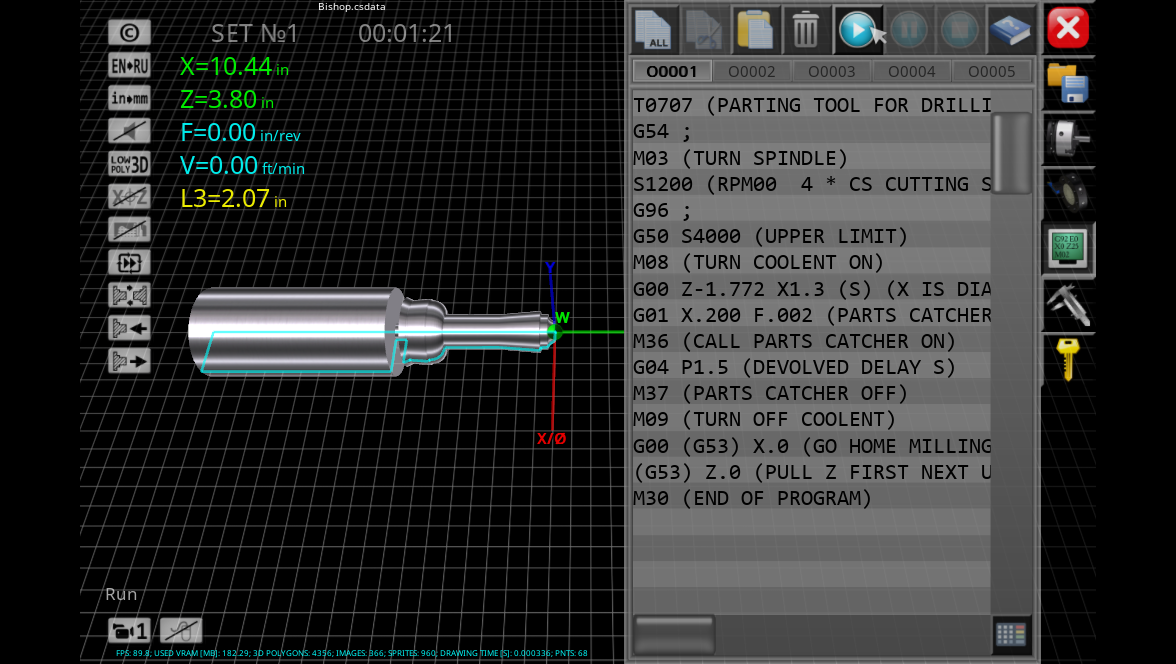
\includegraphics[width=\linewidth]{img/prj05-cnc_simulator_result.png}
\vfill
\end{landscape}

\chapter{Verification of operations in Mastercam}
\begin{landscape}
\vfill
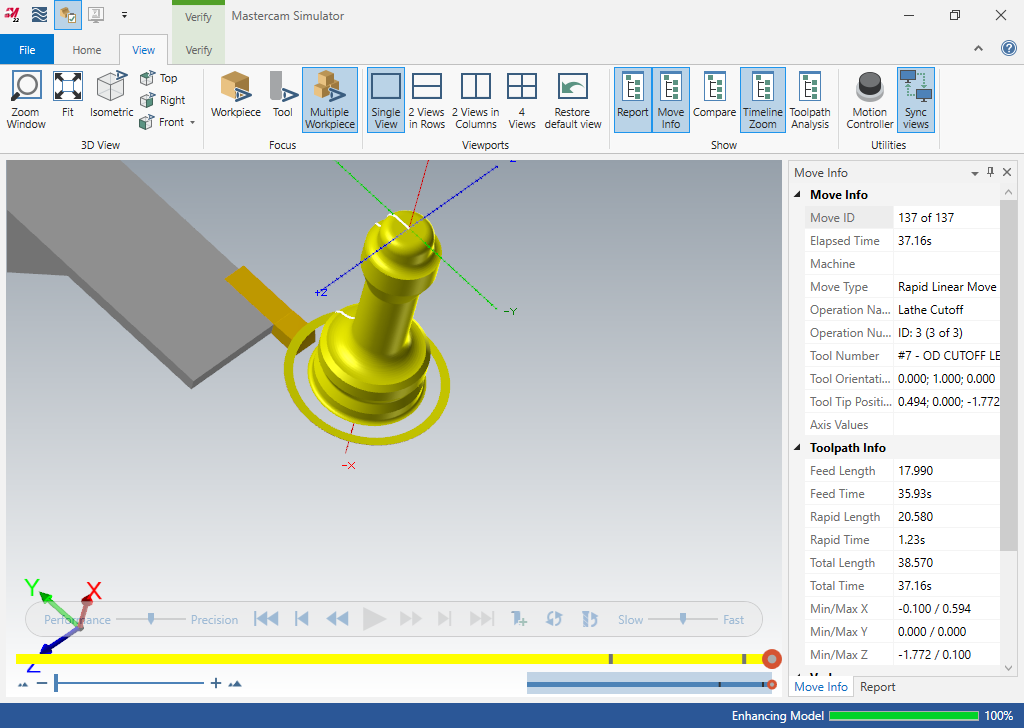
\includegraphics[width=\linewidth]{img/prj05-mastercam_simulator-verification.png}
\vfill
\end{landscape}

%\chapter{Gcode for CNC Simulator}
\addtocounter{chapter}{1}
\includepdf[pages=2-,pagecommand={}]{gcode-cam.pdf}

\chapter{Plot of MasterCAM-generated Gcode in NCViewer}
\begin{landscape}
% this image has a lower portrait aspect ratio than a page, so use height for reference
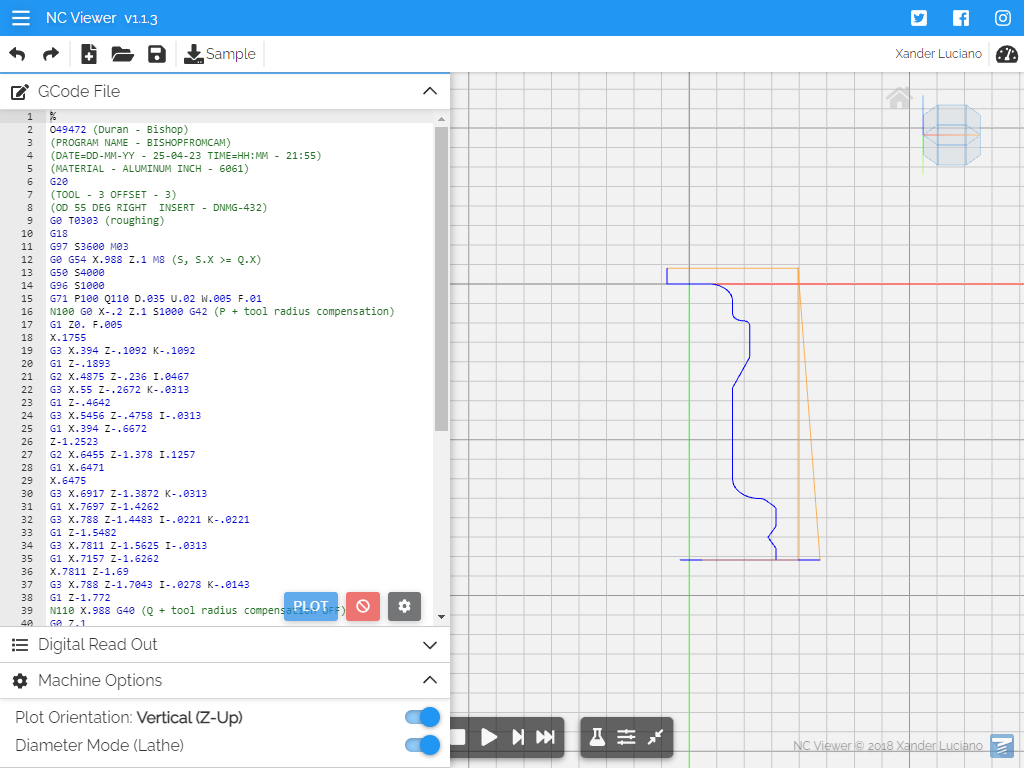
\includegraphics[height=\textheight]{img/prj05-cam-gcode-ncviewer-plot-xz.png}
\end{landscape}

\end{document}
